\section{Interactive sessions}

%
% The idea I am going with for this section is to introduce a few
% filters. Give the audience a suggested image to load, to experiment
% with the filters as they are being describe. Then pose a problem
% which uses the prior filters for them to solve.
%

\subsection{Example}
\begin{frame}{Hands On}
\fontsize{36pt}{36pt}\selectfont
\center
\begin{center}
Interactive Sessions
\end{center}
\end{frame}

\subsection{Threshold-based Segmentation}

\begin{frame}[fragile]
\frametitle{Data To Interact With}
\lstpython
\begin{lstlisting}
# Read image, using ipython's tab auto-complete
image = sitk.ReadImage( ``~/SimpleITK-MICCAI-2011-Tutorial/iasem-cells.nrrd'' )

# Get familiar with the image
print image
...
sitk.Show( image )
\end{lstlisting}
\begin{itemize}
  \item ``Dual-Beam'' or Ion-Abrasion Scanning Electron Microscope
  \item Heavily pre-proccessed
  \item  X-Z cross-section of a 3D volume
\end{itemize}
\end{frame}

\begin{frame}{Image Masks or Binary Images}
Image masks are just SimpleITK Images
\begin{itemize}
  \item Follow some conventions
  \item Pixel type of \texttt{uint8\_t}
  \item 0-value is background, 1-value being the foreground
  \item Masks are used for output of thresholding, binary morphology, etc\dots
  \item The 1-value was choosen to each of computataion with operators
  \item If a mask needs to be directly shown, multiply by 255
\end{itemize}
\end{frame}



\begin{frame}[fragile]
\frametitle{Threshold-based Segmentation}

\begin{itemize}
  \item {\bf Threshold}\\
    \small
    $ Output(x_i) =
    \begin{cases} Input(x_i) &\text{if $Lower \leq x_i \leq Upper$;}  \\
      OutsideValue            &\text{otherwise.}
    \end{cases} $
    \normalsize
  \item {\bf BinaryThreshold}\\
    \small
    $ Output(x_i) =
    \begin{cases} InsideValue &\text{if $LowerThreshold \leq x_i \leq UpperThreshold$;}  \\
      OutsideValue            &\text{otherwise.}
    \end{cases} $
    \normalsize
  \item {\bf OtsuThreshold} - Automatic Threshold values based on minimizing intra-class variance.
  \item {\bf DoubleThreshold} - A morphology based filters. Uses two sets of thresholds.
\end{itemize}

\lstpython
\begin{lstlisting}
# quick visualizations of masked image
sitk.Show( image * mask )
sitk.Show( .5*image*~mask+image*mask )
\end{lstlisting}

\end{frame}


\begin{frame}{Advanced Geodesic Morphology}

\begin{itemize}
  \item {\bf BinaryOpeningByReconstruction} - Removes binary elements which are smaller than the structuring element.
  \item {\bf BinaryClosingByReconstruction} - Fills binary holes which are smaller then the structuring element.
  \item {\bf BinaryFillHole} - Fills all holes in image.
  \item {\bf BinaryGrindPeak} - Removes all binary elements not connected to boarder.
\end{itemize}

\end{frame}

\begin{frame}{Change Border Problem}
Problem:
\begin{itemize}
  \item Registration leaves a border in the image
  \item Border value is average intensity
  \item Change to 0
\end{itemize}
\end{frame}

\begin{frame}{Change Border Solution}
To iPython (\texttt{Examples/InteractiveTutorial/05-01-BorderChange.py})
\end{frame}

\subsection{Numpy Interface}
\begin{frame}[fragile]
\frametitle{SimpleITK with Numpy}

Numpy is:
\begin{itemize}
  \item Python's universal numerics foundation
  \item Provides high performance basic linear algebra
\end{itemize}

numpy interface functions:
\lstpython
\begin{lstlisting}
def GetArrayFromImage(image):
    """Get a numpy array from a SimpleITK Image."""

def GetImageFromArray( arr ):
    """Get a SimpleITK Image from a numpy array."""
\end{lstlisting}
\begin{itemize}
  \item Both of these methods do a deep copy of the image
  \item Ensures safety, bypassing error-prone memory issues
\end{itemize}

\end{frame}

\begin{frame}{Python Example}
To iPython (\texttt{Examples/InteractiveTutorial/05-02-Numpy.py})
\end{frame}

\subsection{Image Measurements}

\begin{frame}{Image Measurements}
\fontsize{36pt}{36pt}\selectfont
\center
\begin{center}
Image Measurements
\end{center}
\end{frame}

\begin{frame}{The Scenerio}
\begin{center}
  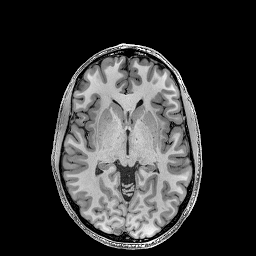
\includegraphics[width=0.3\textwidth]{Images/T1}
  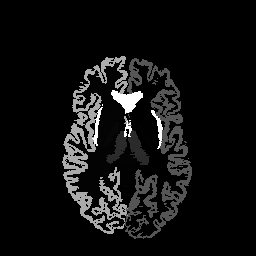
\includegraphics[width=0.3\textwidth]{Images/LB}
  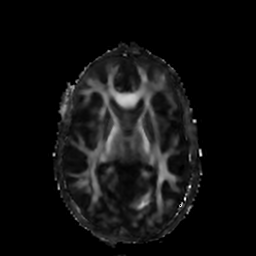
\includegraphics[width=0.3\textwidth]{Images/FA}
\end{center}

\begin{itemize}
  \item You collected 1000 Diffusion Weighted Imaging scan sessions
  \item Now, compute the fractional anisotropy measures for a set of anatomical regions
\end{itemize}
\end{frame}

\begin{frame}{Python Example}
To iPython (\texttt{Examples/InteractiveTutorial/MeasureRegions.py})
\end{frame}

% \begin{frame}[fragile]{Label Statistics}
% \lstpython
% \begin{lstlisting}
% import SimpleITK as sitk
% import csv
% # Load the Images to be measured
% ScalarValuesFile = '~/SimpleITK-MICCAI-2011-Tutorial/FA.png'
% ScalarValuesImage = sitk.Cast( sitk.ReadImage(ScalarValuesFile), sitk.sitkUInt32 )

% LabelMapFile = '~/SimpleITK-MICCAI-2011-Tutorial/LB.png'
% LabelMapImage = sitk.Cast( sitk.ReadImage(LabelMapFile), sitk.sitkUInt32 )

% lsfilter = sitk.LabelStatisticsImageFilter()
% lsfilter.Execute(LabelMapImage,ScalarValuesImage)
% keys = lsfilter.GetValidLabels()

% \end{lstlisting}
% \end{frame}


% \begin{frame}[fragile]{Export Data Table }
% \lstpython
% \begin{lstlisting}
% ### Now extract measurement values to cataloging in a database/spreadsheet
% MySubjectID=``Subj01''
% measurementDict=dict()
% for labelValue in keys:
%   uniqueId = ( MySubjectID, labelValue )
%   measurementMap=lsfilter.GetMeasurementMap(labelValue)
%   measurementDict[uniqueId]=dict( measurementMap )

% print("DUMPING MEASUREMENT DICTIONARY")
% print(measurementDict)
% #A map between internal labels and header row strings.
% headerMap={'SUBJID':'SubjectID',
%            'LABELID':'LabelID',
%            'Variance':'Variance',
%            'Minimum':'Minimum',
%            'Maximum':'Maximum',
%            'Mean':'Mean',
%            'Count':'NumPixels',
%            'approxMedian':'Median',
%            'Sum':'Sum',
%            'Sigma':'Sigma'}

% \end{lstlisting}
% \end{frame}

% \begin{frame}[fragile]{Export Data Table }
% \lstpython
% \begin{lstlisting}

% csvFileName="MyValues.csv"
% csvFile=open(csvFileName, 'wb')
% myDictWriter=csv.DictWriter(csvFile,headerMap.keys())
% myDictWriter.writerow(headerMap)
% for uniqueId in measurementDict.keys():
%   unrollRow = measurementDict[uniqueId]
%   unrollRow['SUBJID']=uniqueId[0]
%   unrollRow['LABELID']=uniqueId[1]
%   myDictWriter.writerow(unrollRow)
% csvFile.close()

% \end{lstlisting}
% \end{frame}

\subsection{Feature Detection}

\begin{frame}{Feature Detection}
\fontsize{36pt}{36pt}\selectfont
\center
\begin{center}
Feature Detection
\end{center}
\end{frame}

\begin{frame}[fragile]
\frametitle{More Data To Interact With}
\lstpython
\begin{lstlisting}
# Read image, using ipython's tab auto-complete
image = sitk.ReadImage( ``~/SimpleITK-MICCAI-2011-Tutorial/iasem-mito.nrrd'' )

# Get familiar with the image
print image
...
sitk.Show( image )
\end{lstlisting}
\end{frame}

\begin{frame}[fragile]
\frametitle{Edge Detection} 

\begin{itemize}
  \item {\bf CannyEdgeDetection}
\begin{lstlisting}
    Image CannyEdgeDetection ( const Image& ,
      double inLowerThreshold = 0.0,
      double inUpperThreshold = 0.0,
      std::vector<double> inVariance = std::vector<double>(3, 0.0),
      std::vector<double> inMaximumError = std::vector<double>(3, 0.01) );
\end{lstlisting}
  \item {\bf SobelEdgeDetection }
\begin{lstlisting}
    Image SobelEdgeDetection ( const Image&  );
\end{lstlisting}
  \item {\bf ZeroCrossingBasedEdge }
\begin{lstlisting}
    Image ZeroCrossingBasedEdgeDetection ( const Image& ,
      double inVariance = 1,
      uint8_t inForegroundValue = 1u,
      uint8_t inBackgroundValue = 0u,
      double inMaximumError = 0.1 );
\end{lstlisting}
  \item {\bf GradientMagnitudeRecursiveGaussian }
\begin{lstlisting}
    Image GradientMagnitudeRecursiveGaussian ( const Image& ,
      double inSigma = 1.0,
      bool inNormalizeAcrossScale = false );
\end{lstlisting}
\end{itemize}

\end{frame}


\begin{frame}[fragile]
\frametitle{Image Derivatives}

\begin{itemize}
  \item {\bf Derivative}
\begin{lstlisting}
    Image Derivative ( const Image& ,
      unsigned int inDirection = 0u,
      unsigned int inOrder = 1u,
      bool inUseImageSpacing = true );
\end{lstlisting}
  \item {\bf RecursiveGaussian}
\begin{lstlisting}
    Image RecursiveGaussian ( const Image& ,
      double inSigma = 1.0,
      bool inNormalizeAcrossScale = false,
      itk::simple::RecursiveGaussianImageFilter::OrderEnumType inOrder = itk::simple::RecursiveGaussianImageFilter::ZeroOrder,
      unsigned int inDirection = 0u );
\end{lstlisting}
\end{itemize}

\end{frame}

\begin{frame}[fragile]
\frametitle{Zero Crossing}
  

\begin{itemize}
  \item {\bf ZeroCrossing }
\begin{lstlisting}
    Image ZeroCrossing ( const Image& ,
      uint8_t inForegroundValue = 1u,
      uint8_t inBackgroundValue = 0u );
\end{lstlisting}
\end{itemize}

\end{frame}


\begin{frame}[fragile]
\frametitle{Ridge and Valley Detection Problem}

Where $g(x;t)$ is a Gaussian function:\\
\center
\begin{equation}
g(x;t) = \frac{ 1 }{ \sqrt{ 2 t \pi } } e^{ \left( - \frac{x^2}{ 2 t} \right) }
\end{equation}
Let $L$ denote a scale-space representaton of an image $I$:\\
\begin{equation}
L(x,y;t) = g(x,y; t) \ast I(x,y)
\end{equation}
And then $L_x$ is the partial derivative of the scale-space
representation of $I$ with respect  to $x$. 
\end{frame}

\begin{frame}[fragile]
\frametitle{Ridge and Valley Detection Problem (continued)}
Derivatives can also be
taken in other, directions. If $v$ is a direction parallel to image
gradient, then the following  defines a ridge:
\begin{equation}
L_{uv} = 0, L_{uu}^2-L^2_{vv} \ge 0
\end{equation}
Where these directional derivatives have the following properties:
\begin{align}
L_v^2L_{uu}&=L_x^2L_{yy}-2L_xL_yL_{xy}+L_y^2L_{xx},\\
L_v^2L_{uv}&=L_xL_y(L_{xx}-L_{yy}) - (L_x^2-L_y^2)L_{xy},\\
L_v^2L_{vv}&=L_x^2L_{xx}+2L_xL_yL_{xy} +L_y^2L_{yy}
\end{align}

This view of the Ridge Detection if taken from Tony Lindeberg's works.

\end{frame}

\begin{frame}{Ridge Detection Example}
To iPython (\texttt{Examples/InteractiveTutorial/05-04-RidgeDetection.py})
\end{frame}




